\subsection{Le moteur audio}

\subsubsection{Présentation des différentes méthodes offertes}

L'une des raisons pour lesquelles nous avons choisi Qt est la
richesse de ses librairies. Deux d'entre elles permettent de gérer le son
: Phonon et QtMultimedia. Phonon a été rapidement abandonnée car
elle est de très haut niveau et plutôt adaptée pour jouer des
fichiers audio et vidéo compressés.

En revanche, QtMultimedia semblait idéale car elle permet de
fournir des buffers directement à la carte son de la même manière
qu'on adresserait un fichier. QtMultimedia propose deux modes de
fonctionnement : en \emph{Pull} ou \emph{Push}.

Nous avons d'abord testé le mode \emph{Pull}, car il semblait bien
adapté à notre séquenceur qui travaille lui aussi en \emph{Pull}.
Malheureusement, nos essais ont montré que si l'implémentation est
remarquablement simple à mettre en place, la gestion de la latence
est mauvaise : celle-ci est instable, le nombre d'octets à fournir
varie de très faible (une centaine d'octets) à très important
(16k). Il est bien sûr possible de stabiliser le tout en passant
par un buffer intermédiaire, mais cela aurait augmenté la latence de
l'application de manière insupportable pour l'utilisateur.

Nous avons alors testé le mode \emph{Push}. À l'inverse, il faut
demander régulièrement à la carte son si elle a besoin de données,
à fournir au travers d'un QIODevice, composant d'entrée/sortie
générique qui les achemine à la carte son. Le principal
inconvénient de cette technique est qu'il faut constamment demander
l'état du buffer de la carte son.

\subsubsection{Base du moteur audio}

Nous avons créé une classe \verb!AudioDeviceProvider!, singleton
qui se charge d'initialiser un QAudioOutput. Ce dernier permet
de trouver un driver audio compatible avec le format désiré,
indiqué dans un \verb!QAudioFormat! (dans notre cas, du 44100Hz, 16
bits, mono). \verb!QAudioOutput! fournit en plus, en mode
\emph{Push}, le \verb!QIODevice! qui servira à envoyer les données
à la carte son par l'intermédiaire de la méthode \verb!write!.
Enfin, le \verb!QAudioOutput! nous renseigne sur le nombre d'octets
dont a besoin la carte son par la méthode \verb!bytesfree!.

Une classe \verb!Clock!, également singleton et créée par nos
soins, se charge d'appeler le séquenceur à intervalle régulier
(toutes les 30 ms). Cela permet à tous les modules qui ont besoin
d'être rafraîchis d'être appelés, même si aucun module
\verb!Speaker! n'est présent. L'oscilloscope, le File Writer, le
WAV Looper et le Sampler notamment sont ainsi actualisés.

En revanche, si un module dit «~\emph{time critical}~»
(typiquement, un module \verb!Speaker!) est placé sur l'interface,
il s'enregistre auprès de la \verb!Clock! dans une liste de timers
rapides (\emph{Fast Timers}), appelés à intervalle très rapide (5
ms). Une fois qu'un module est enregistré dans cette liste, le
séquenceur n'est plus appelé par le thread non critique. Ce sera de nouveau le
cas si les modules inscrits dans les timers rapides se
désinscrivent.

Le traitement des \emph{Fast Timers} est alors différent, comme
expliqué plus loin.

\subsubsection{\emph{Push} : technique non utilisée}

La technique de base, qui s'avérait être la plus propre d'un point
de vue architecture, n'a pas été retenue dans l'implémentation
finale, car nous n'avons jamais pu obtenir un résultat correct en
sortie (son qui «~saute~»), malgré les traces que nous avons
implanté et montrant un acheminement correct des informations.

\begin{figure}[ht]
\centering
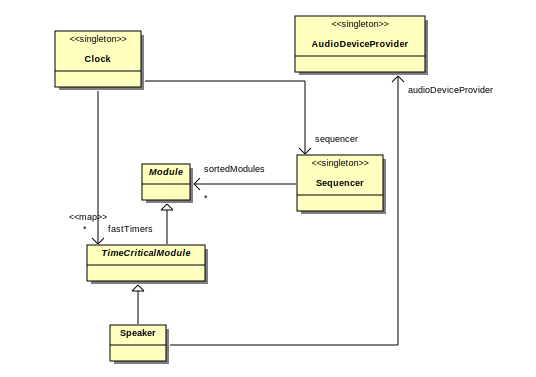
\includegraphics[width=17cm]{../img/ps/psm_unusedAudioEngine.pdf}
\caption{Diagramme de séquence du moteur audio inutilisé car non fonctionnel}
\label{fig:unused-audioengine}
\end{figure}

La figure \ref{fig:unused-audioengine} illustre cette technique.
Lorsque le \emph{Fast Timer} est écoulé, la \verb!Clock! vérifie si
la carte son a besoin d'être alimentée. Si c'est le cas, le
séquenceur est appelé une fois. On recommence l'appel au séquenceur
tant que la carte son a besoin de données (avec une limite
arbitraire de 10 itérations). Lors de l'appel au séquenceur,
celui-ci appelle la fonction \verb!process()! du module
\verb!Speaker!.

Celui-ci dispose d'un buffer circulaire qui contient des données
formatées pour être envoyées à la carte son (format char, little
endian). L'appel à \verb!process()! ayant au préalable mis à jour
les entrées du module \verb!Speaker!, il est important de les
ajouter directement au buffer circulaire. On alimente ensuite la
carte son avec les données possédées et dont elle a besoin. Si la
quantité est insuffisante, au retour de l'appel la boucle de
\verb!Clock! rappellera de nouveau le séquenceur qui appellera de
nouveau le \verb!process()! de chaque module, dont \verb!Speaker!.

La théorie et les traces fonctionnent parfaitement. Pour des
raisons que nous n'avons pas pu déterminer, la pratique laisse à
désirer, de nombreuses coupures venant s'intercaler dans le flux
audio généré. Nous avons donc tenté une autre approche, moins
propre d'un point de vue architecture car non symétrique, mais
cependant fonctionnelle.

QtMultimedia étant une librairie très récente, il ne nous a pas été
possible de trouver une explication à nos divers problèmes (mode
\emph{Pull} à latence instable, mode \emph{Push} avec des pertes
selon la technique) sur les divers forums visités.

\subsubsection{\emph{Push} : technique utilisée}

\begin{figure}[ht]
\centering
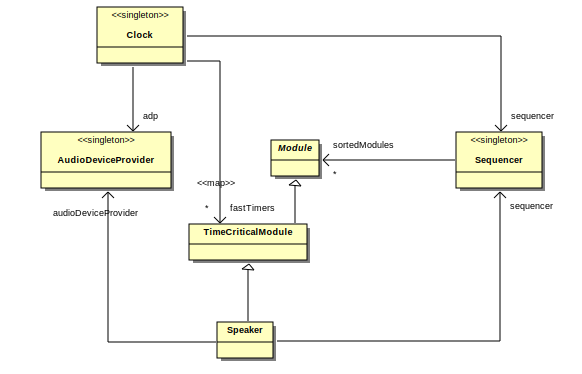
\includegraphics[width=17cm]{../img/ps/psm_currentAudioEngine.pdf}
\caption{Moteur Audio utilisé par l'application}
\label{fig:audioengine}
\end{figure}

La figure \ref{fig:audioengine} illustre la technique utilisée,
elle consiste à déléguer la gestion complète de la
carte son au module \verb!Speaker!. La \verb!Clock! dispose
toujours du même mécanisme de timers normaux/critiques, mais le
timer critique appelle le \emph{slot} \verb!fastTimerExpired()! de
chaque module. Cela permet de découpler l'appelant de l'appelé.

Une fois le slot \verb!fastTimerExpired()! du \verb!Speaker!
appelé, on vérifie dans une boucle si la carte son a besoin de
données. Si oui, on appelle le séquenceur à partir du
\verb!Speaker! et on envoie directement le buffer d'entrée du
module vers la carte son. Si celle-ci a encore besoin de données,
on réitère la boucle, avec une limite arbitraire de 10 itérations.
La figure \ref{fig:audioengine-sequence} montre les ces échanges.

\begin{figure}[p]
\centering
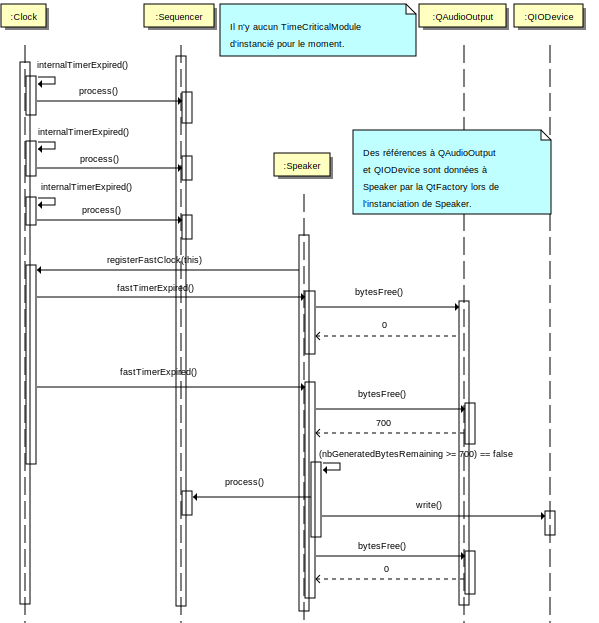
\includegraphics[width=17cm]{../img/ps/psm_currentAudioEngine_Sequence.pdf}
\caption{Diagramme de séquence du moteur audio utilisé}
\label{fig:audioengine-sequence}
\end{figure}

L'inconvénient de cette méthode est que, sans module critique,
c'est la \verb!Clock! qui appelle le séquenceur, mais avec un
module critique, c'est le module lui-même qui appelle le séquenceur
en fonction de ses besoins. L'appel au séquenceur est donc
asymétrique. Afin que seuls les modules critiques puissent être
appelés par \verb!Clock!, et pour éviter que les modules aient à
implémenter des méthodes qu'ils n'utiliseront jamais, nous avons
dérivé \verb!Module! en \verb!TimeCriticalModule!, dont seules les
instances implémentent le \emph{slot} \verb!fastTimerExpired!. En
conséquence, les méthodes \verb!registerFastTimer! et
\verb!unregisterFastTimer! de \verb!Clock! n'accepteront que des
\verb!TimeCriticalModule!.

L'avantage de cette méthode est indéniable : elle fonctionne en
pratique. La latence est très faible et le son stable.
